\documentclass{minimal}
\usepackage[margin=2cm,landscape,a3paper]{geometry}
\usepackage{tikz}
\usepackage{pgfplots}
\usepackage{pst-node}
\usetikzlibrary{calc}
\usetikzlibrary{decorations.text}

\def\centerarc[#1](#2)(#3:#4:#5)% Syntax: [draw options] (center) (initial angle:final angle:radius)
    { \draw[#1] ($(#2)+({#5*cos(#3)},{#5*sin(#3)})$) arc (#3:#4:#5); }

\begin{document}
\begin{tikzpicture}

\definecolor{blueee}{RGB}{61,98,148}
\definecolor{greenn}{RGB}{113,191,110}
\definecolor{orangee}{RGB}{255,153,51}
\definecolor{redd}{RGB}{233,72,73}
\definecolor{darkbluee}{RGB}{44,68,120}
\definecolor{darkgreenn}{RGB}{100,165,95}
\definecolor{darkorangee}{RGB}{126,72,25}
\definecolor{darkredd}{RGB}{116,36,36}

\node[inner sep=0pt] (phantom) at (0,-0.35)
    {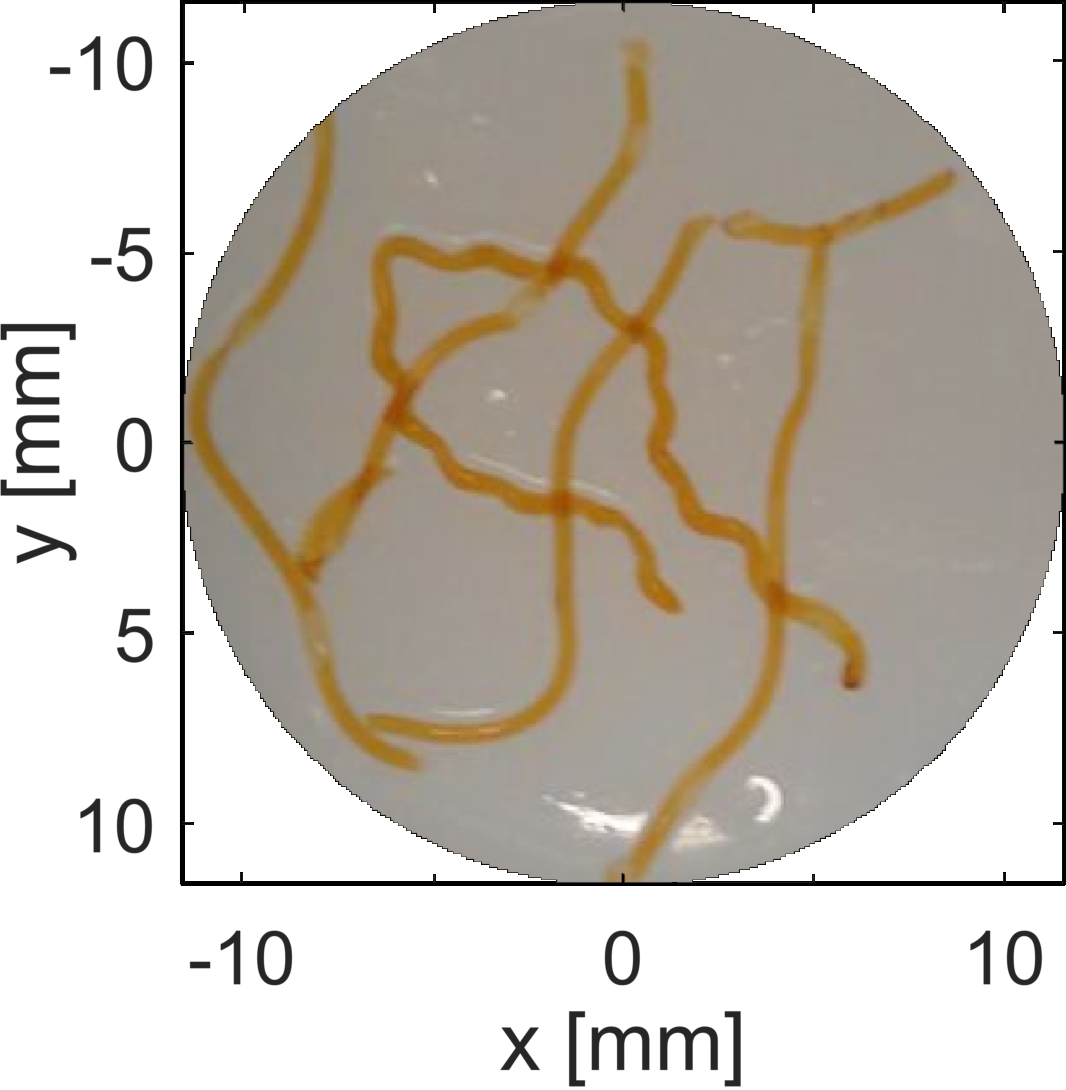
\includegraphics[width=7.5cm]{experimental_photo2.png}};


\node[inner sep=0pt] (phantom_zoom) at (10,0)
    {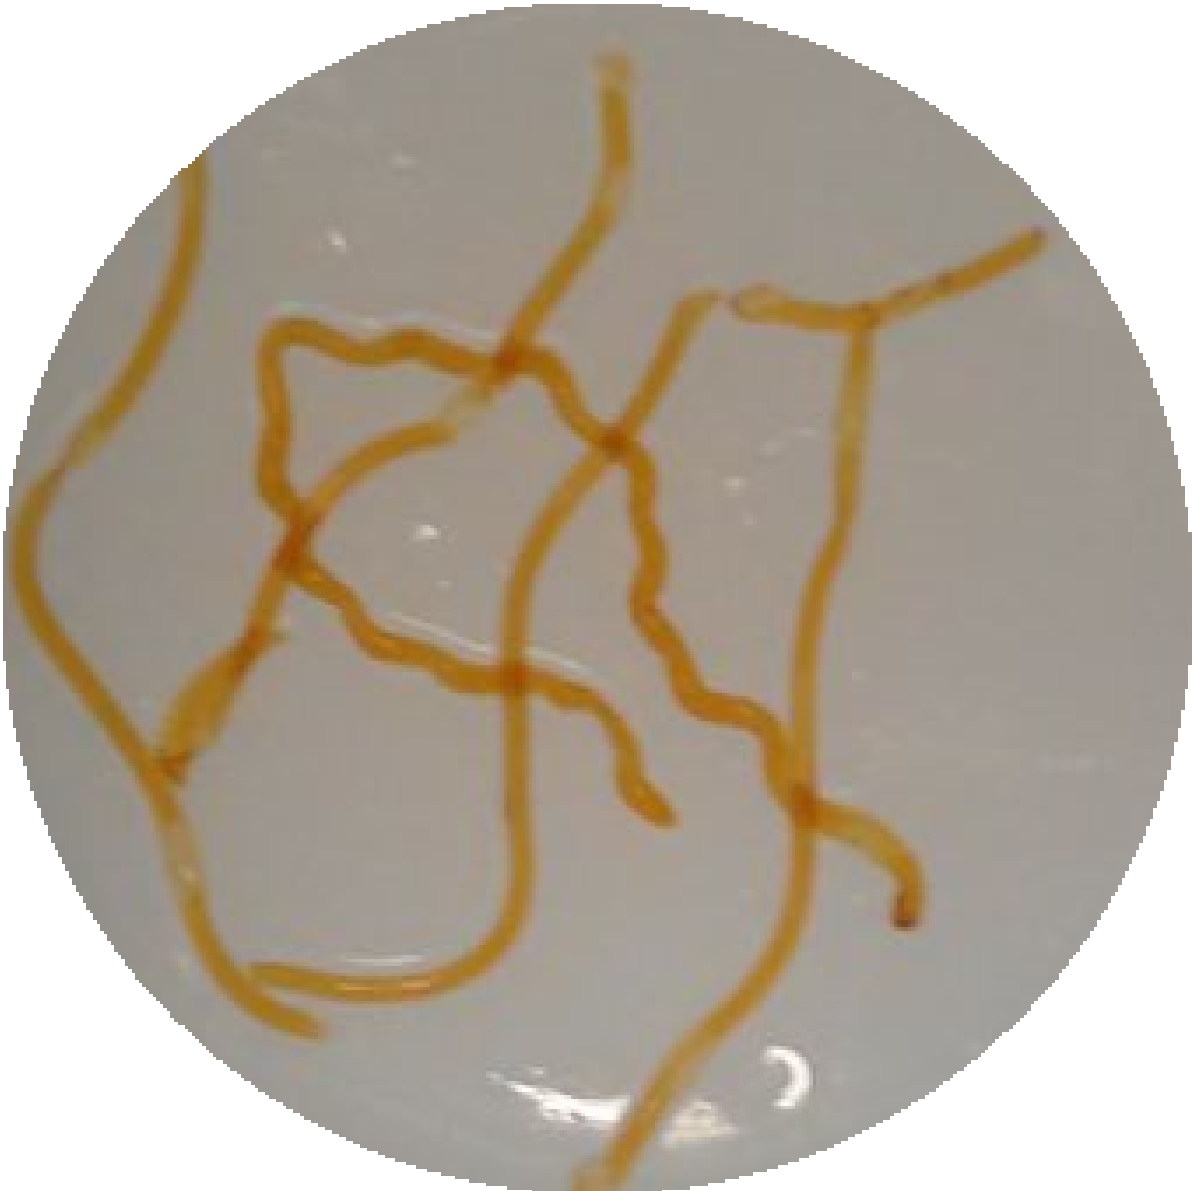
\includegraphics[width=2.5cm]{exp_phantom.png}};

\foreach \i in {0,...,31}
{
	\centerarc[darkgreenn,line width=2.0](10,0)(11.25*\i-(1.40625+0.703+0.1):11.25*\i+1.50625-(1.40625+0.703):4.0)
}
    
\foreach \i in {0,...,63}
{
	\centerarc[black,line width=2.0](10,0)(5.625*\i-(1.40625+0.703):5.625*\i+1.40625-(1.40625+0.703):3.75)
}

\foreach \i in {1,...,32}
{
	\centerarc[redd,line width=1.6](10,0)(45+2.8125*\i-(1.40625+0.703):45+2.8125*\i+1.40625-(1.40625+0.703):3.25)
}

\foreach \i in {1,...,64}
{
	\centerarc[blueee,line width=1.6](10,0)(2.8125*\i-(1.40625+0.703):2.8125*\i+1.40625-(1.40625+0.703):3.5)
}


%\draw[darkgreenn, line width=2.0] (16,2)--(16.5,2);
\draw[black, line width=0.5] (1.2,-2.71)--(10.2,-1.26);
\draw[black, line width=0.5] (1.2,3.44)--(10.2,1.24);

\end{tikzpicture}
\end{document}